\documentclass[../Article_Model_Parameters.tex]{subfiles}
\graphicspath{{\subfix{../Figures/}}}
\begin{document}
	
	\label{CH: Results}
	
	The sensitivity equations were solved simultaneously with the original process model. The focus of this work is to investigate the influence of inlet temperature, pressure and mass flow-rate on the state-space as wall as on the extraction yield. 
	
	\subsection{Flow-rate}
	
	The increase of the mass-flow rate affects the whole system simultaneously in the spatial direction. The change in mass flow-rate makes the fluid moves faster, but its thermodynamic state is not affected. As the result, Figure \ref{fig:Sensitivty_F_P} show no change in pressure during the simulation. 
    
    \begin{figure}[h!]
    	\centering
    	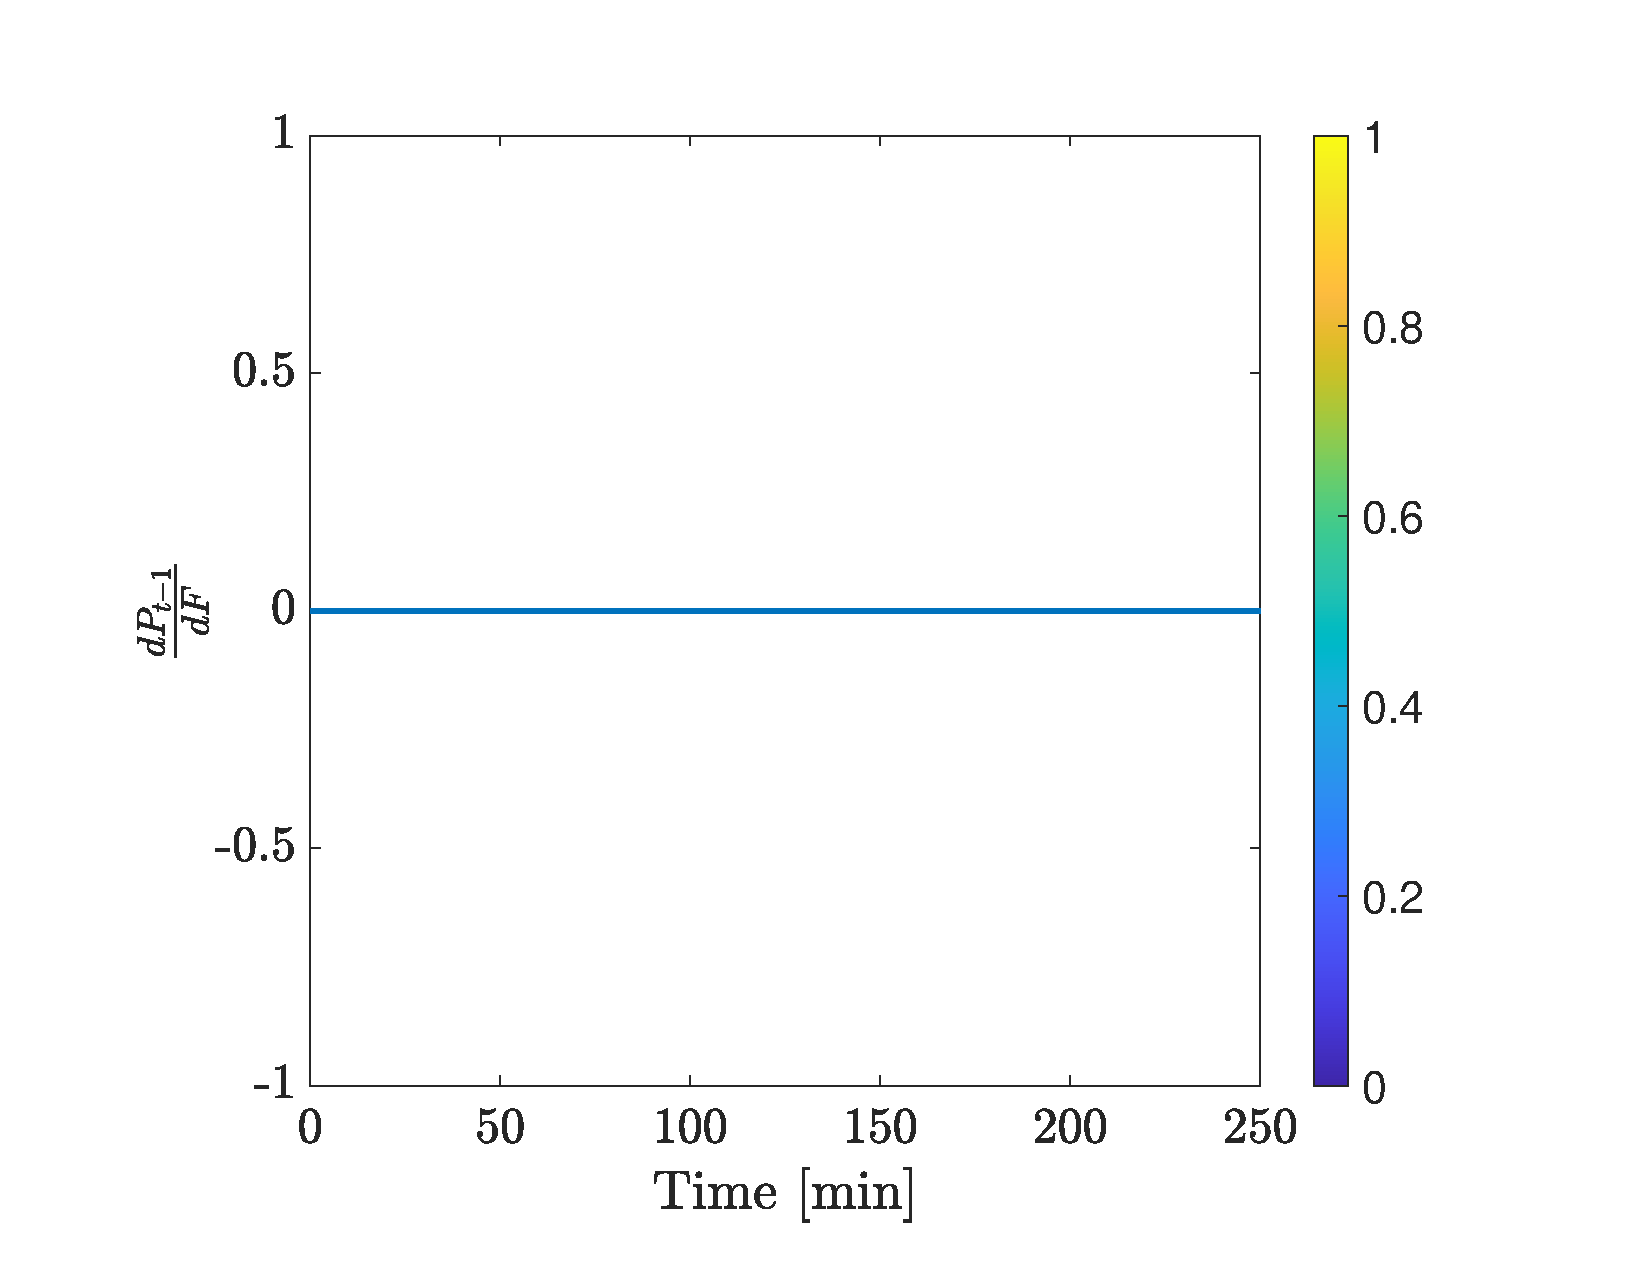
\includegraphics[trim = 2cm 0cm 0cm 0cm,clip,width=\columnwidth]{/Results_sensitivity/P_F.pdf}
    	\caption{The effect of $F$ change on $P$}
    	\label{fig:Sensitivty_F_P}
    \end{figure}
    
    Similarly, the energy in the system (defined as $\rho \times h$) is not affected as presented on Figure \ref{fig:Sensitivty_F_H}. As pressure and temperature are not affected by the increase in the mass flow-rate, the fluid density $\rho$ and enthalpy $h$ are insensitive to flow-rate change.
    
    \begin{figure}[h!]
    	\centering
    	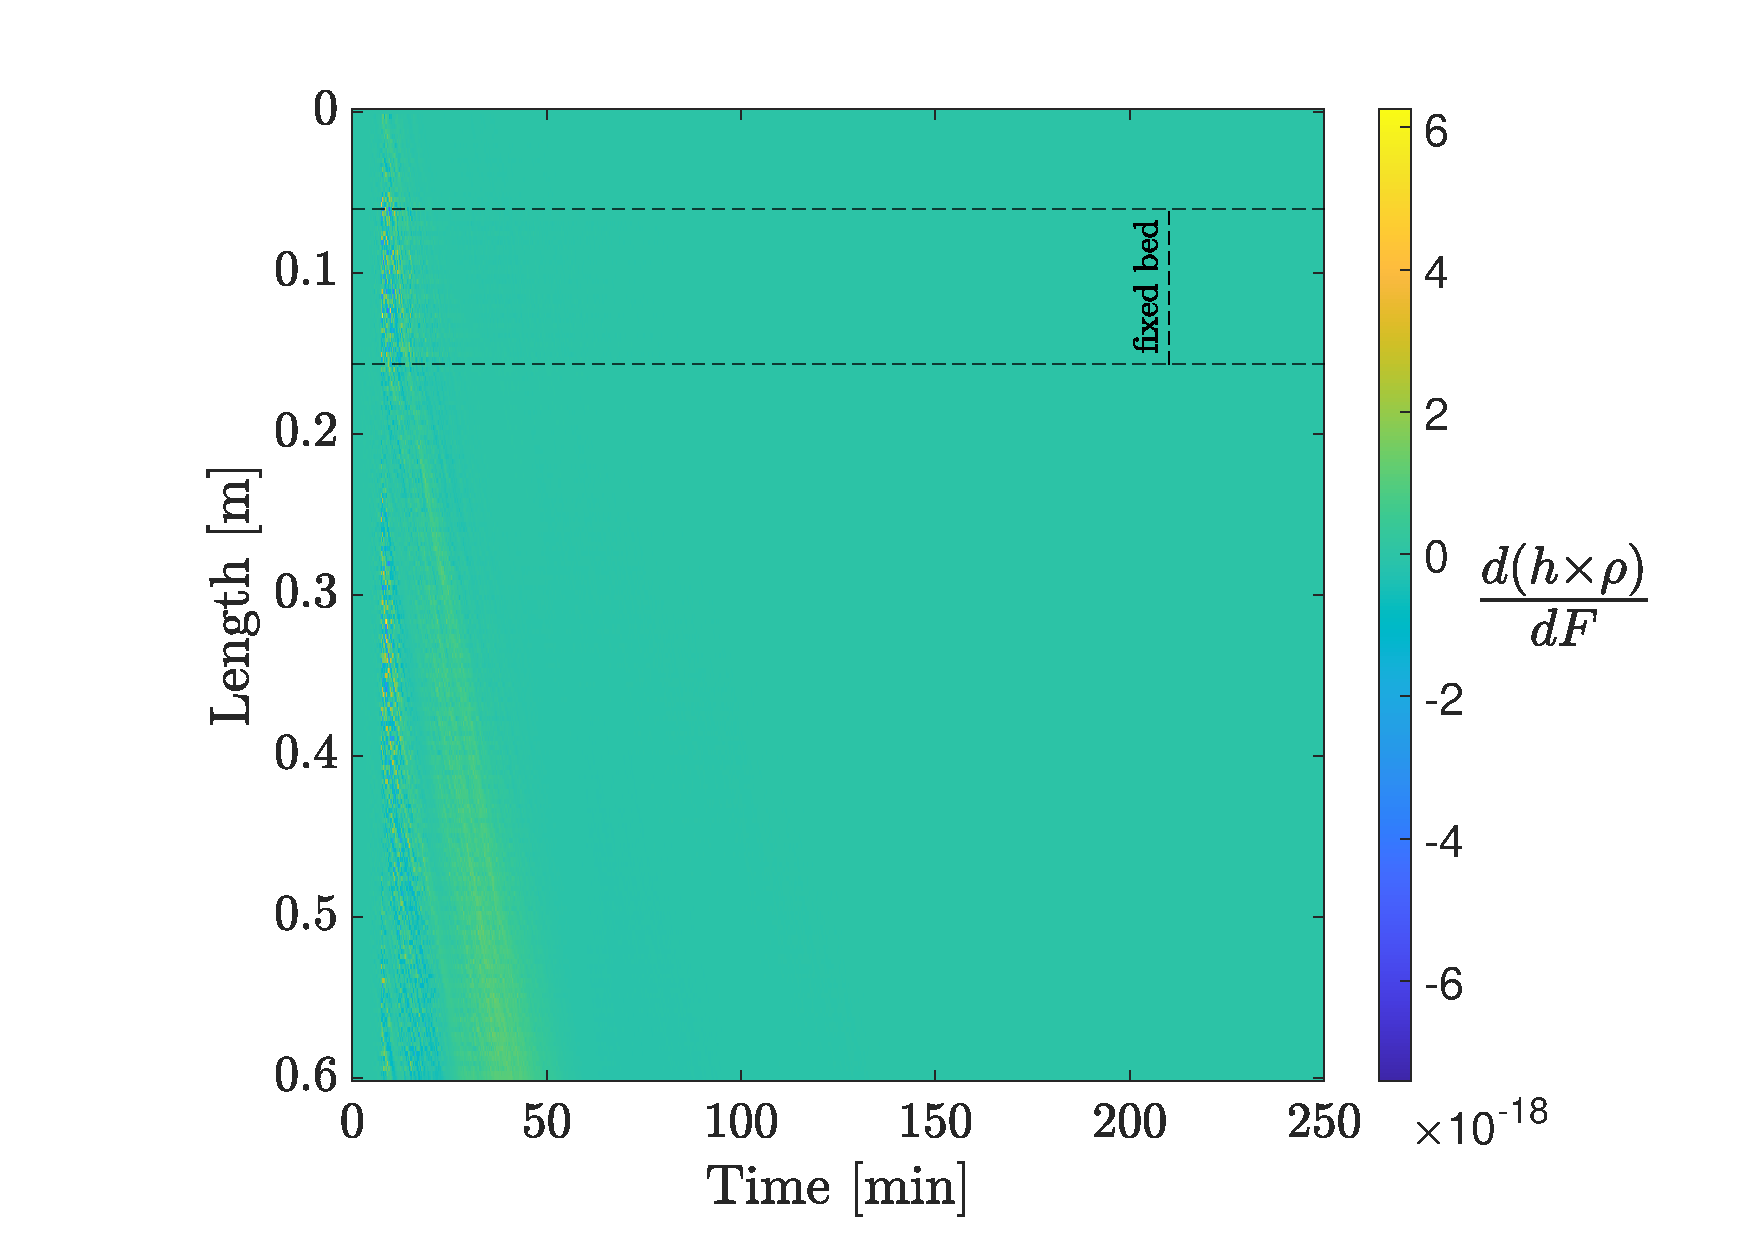
\includegraphics[trim = 2cm 0cm 0cm 0cm,clip,width=\columnwidth]{/Results_sensitivity/H_F.pdf}
    	\caption{The effect of $F$ change on $\rho \times h$}
    	\label{fig:Sensitivty_F_H}
    \end{figure}
    
    The increase in the mass flow rate affects the concentration gradient and accelerates the extraction kinetics. Negative sensitivities in Figure \ref{fig:Sensitivty_F_CS} present the faster extraction rate. Negative values of $dc_s/dF$ can be interpreted as a 'faster' mass loss from the solid phase, which means the extraction efficiency improves. At the beginning of the extraction process, the change in the flow rate has a minimal effect on the extraction process (represented by close to zero sensitivities), due to the high concentration gradient, which leads the extraction kinetic. Later, the increment of the mass flow rate accelerates the extraction kinetic and sensitivities along the decrease to minimum values. Over time, the amount of solute in the solid phase decreases, and eventually, the extraction kinetic becomes limited by the concentration gradient. This behaviour is represented by sensitivities, which asymptotically go to zero. The asymptotic movement of sensitivities can be explained by the fact that the increase in the flow rate does not affect the extraction if all the solute has been removed from the solid phase.
    
    \begin{figure}[h!]
    	\centering
    	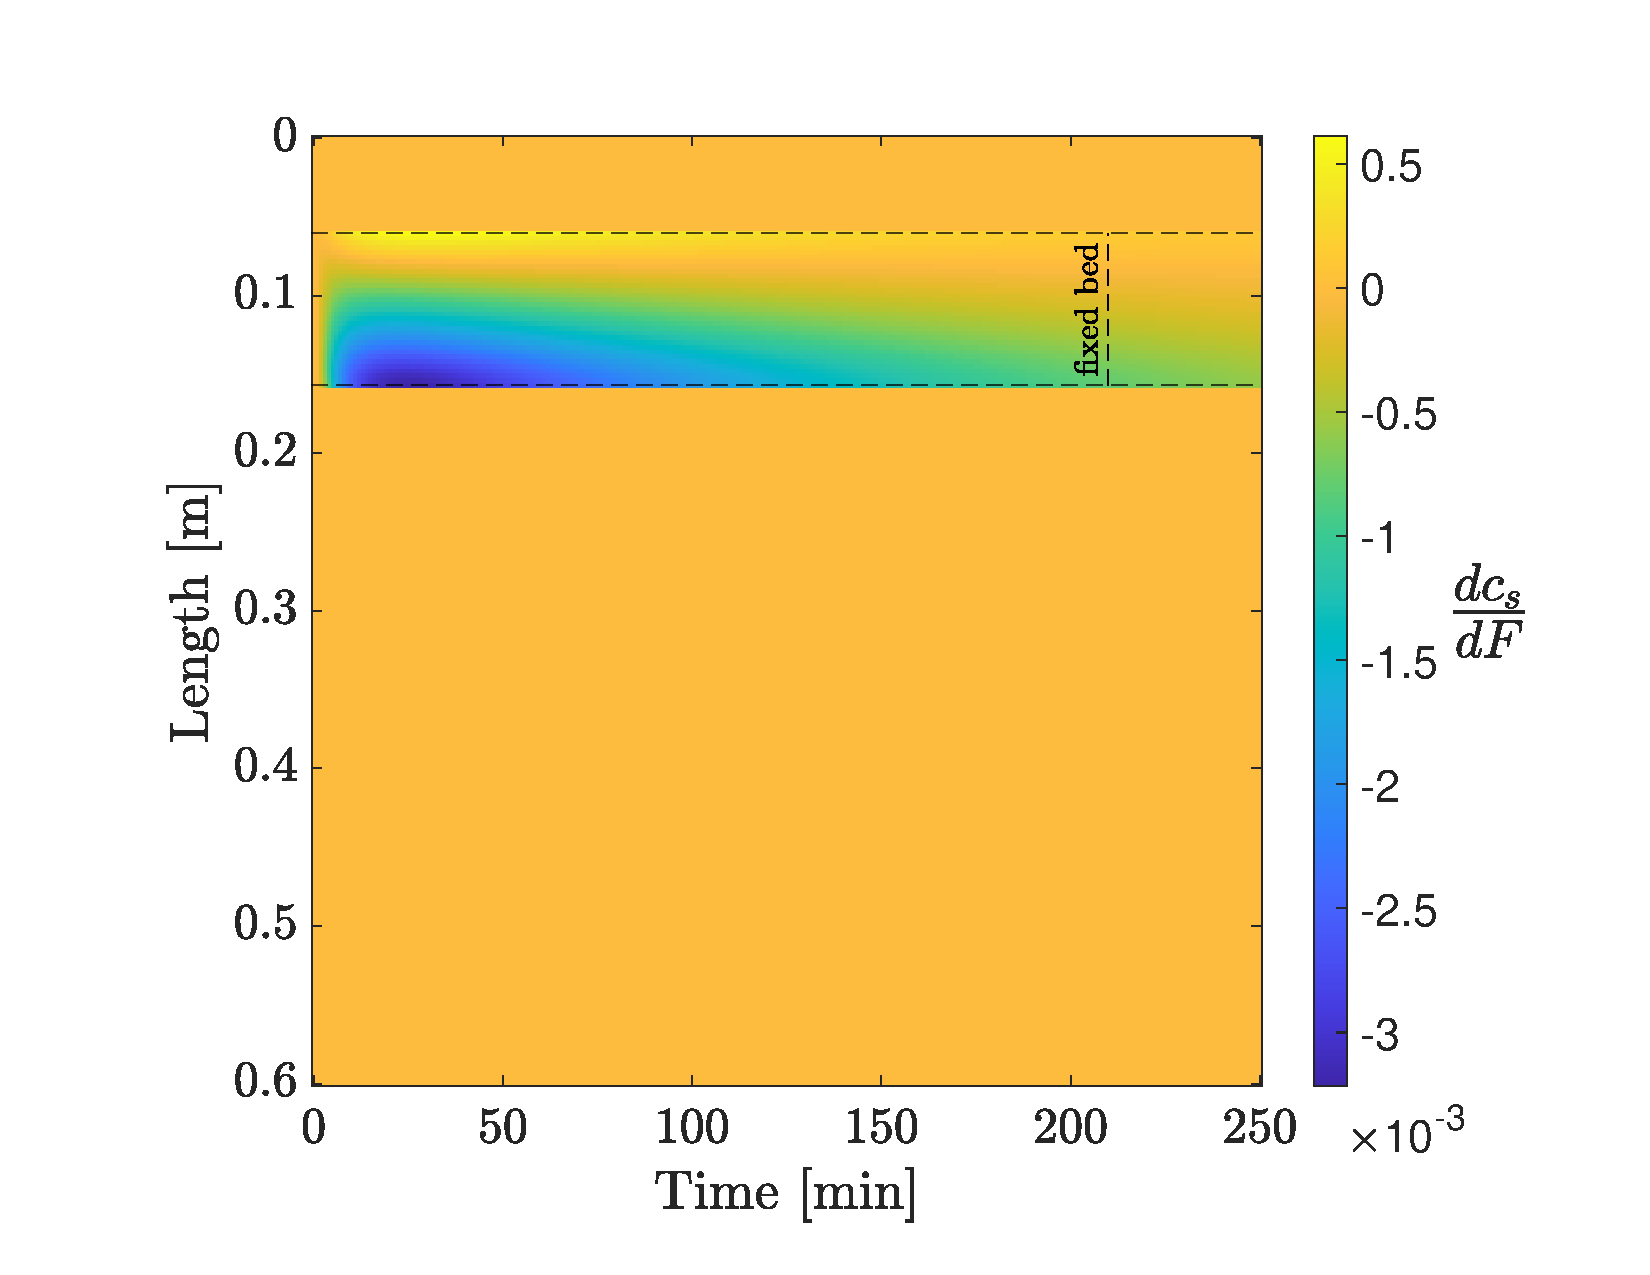
\includegraphics[trim = 2cm 0cm 0cm 0cm,clip,width=\columnwidth]{/Results_sensitivity/CS_F.pdf}
    	\caption{The effect of $F$ change on $C_s$}
    	\label{fig:Sensitivty_F_CS}
    \end{figure}
    
    Figure \ref{fig:Sensitivty_F_CF} shows how the concentration of solute in the fluid phase is affected by the flow-rate increment. Initially, sensitivities are close to zero, which indicates very little system response. The flow-rate growth affects the ${\color{blue}C_f}(z,t)$ by increasing the velocity of the solute across the system, which also increases the concentration gradient. As a result, the positive sensitivities appear in the system and form a front, which moves from the inlet to the outlet of the extractor. Because the larger amount of solute moves faster across the system, the total amount of solute in both phases decreases faster, which eventually causes negative sensitivities to appear in the system. The negative sensitivities form the second front, which moves across the extractor. Eventually, the negative sensitivities asymptotically go to zero.
    
    \begin{figure}[h!]
    	\centering
    	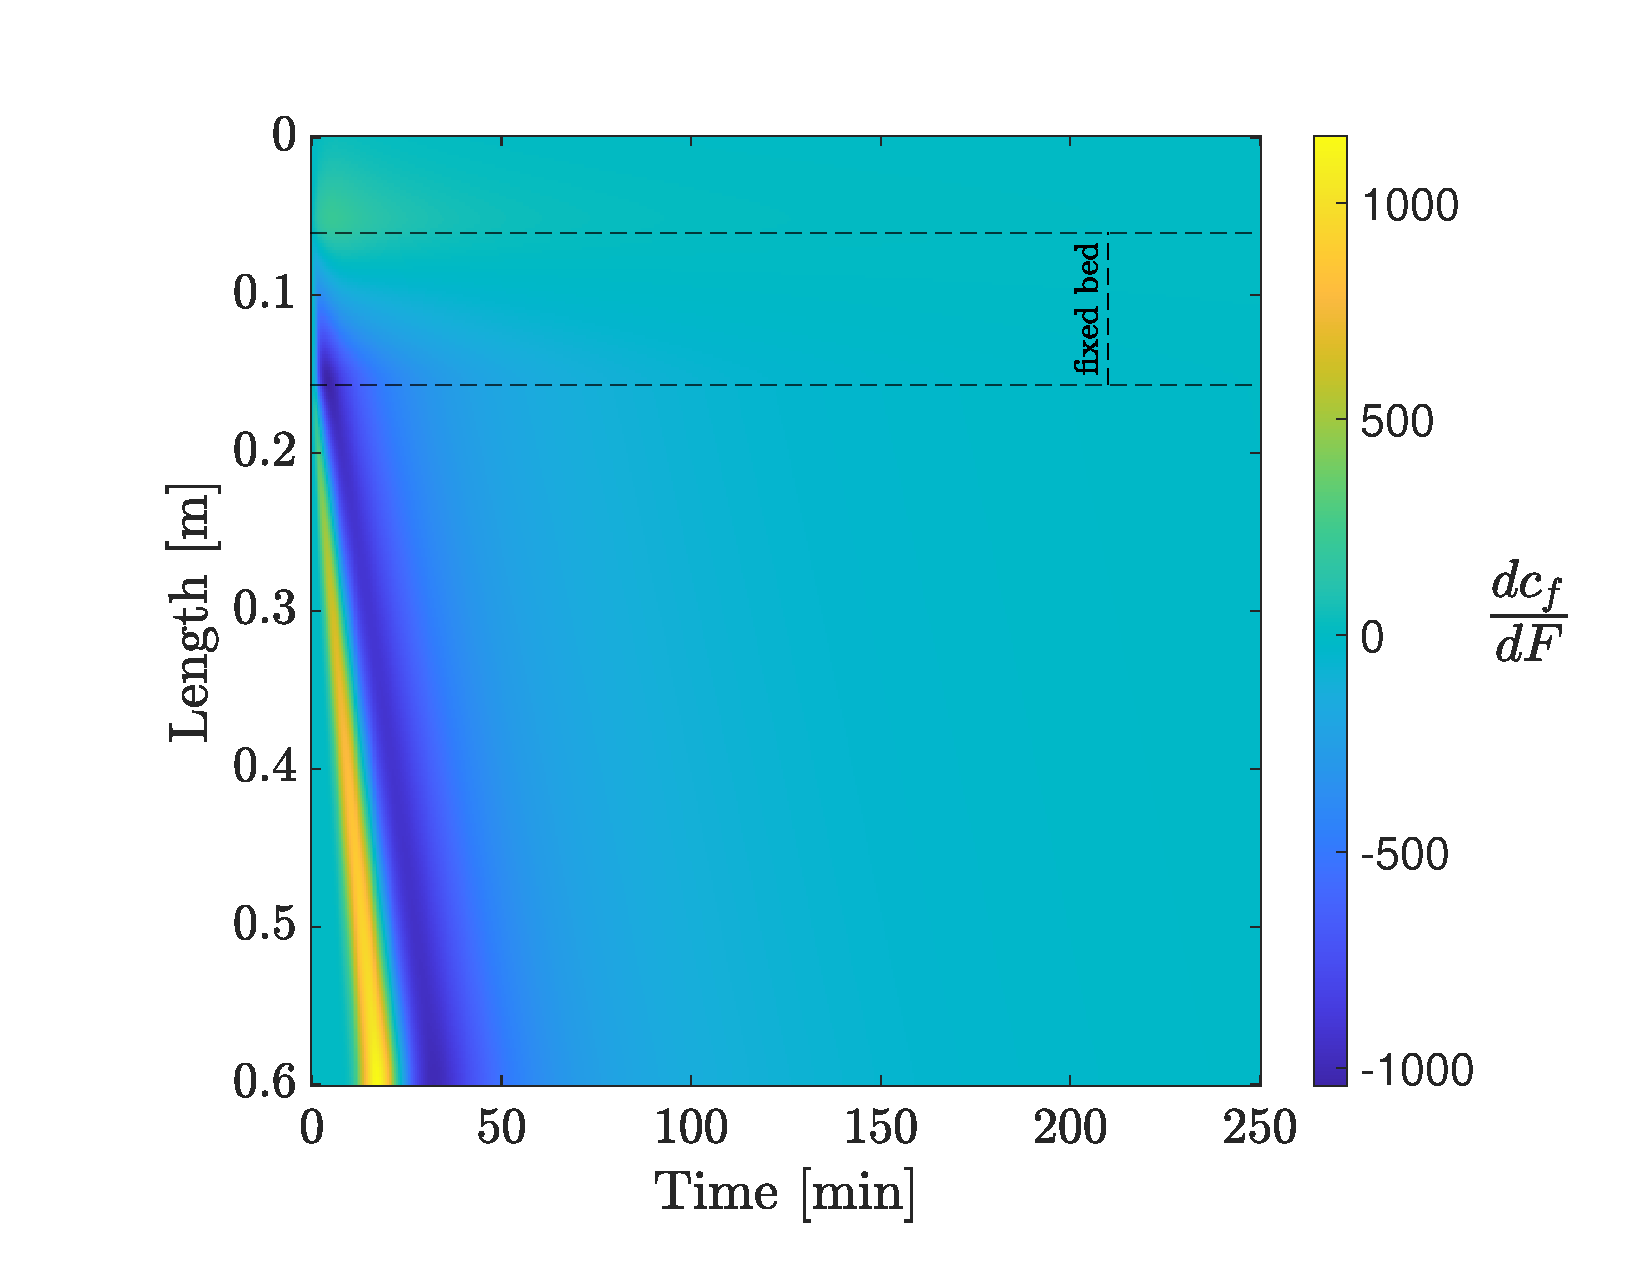
\includegraphics[trim = 2cm 0cm 0cm 0cm,clip,width=\columnwidth]{/Results_sensitivity/CF_F.pdf}
    	\caption{The effect of $F$ change on $C_f$}
    	\label{fig:Sensitivty_F_CF}
    \end{figure}
    
    Figure \ref{fig:Sensitivty_F_y} shows how the flow-rate increment changes the extraction yield. Initially, the sensitivity curve stays flat, which is caused by the fact that the fixed bed does not occupy the whole volume of the extractor, and the fluid needs some time to flow through the empty part of the extractor to reach its outlet. When the solute in the fluid phase reaches the outlet of the extractor, then system response can be observed. The $dy/dF$ starts to increase, and positive value of sensitivity indicates an improvement in the process efficiency, hence the yield increment. Over time, the sensitivity reaches its maximum and diminishes due to decreasing concentration gradient. The $dy/dF$ asymptotically goes to zero because the amount of solute in the fluid phase becomes a limiting factor of the extraction process, and the flow-rate increment has less effect on the extraction yield.
    
    \begin{figure}[h!]
    	\centering
    	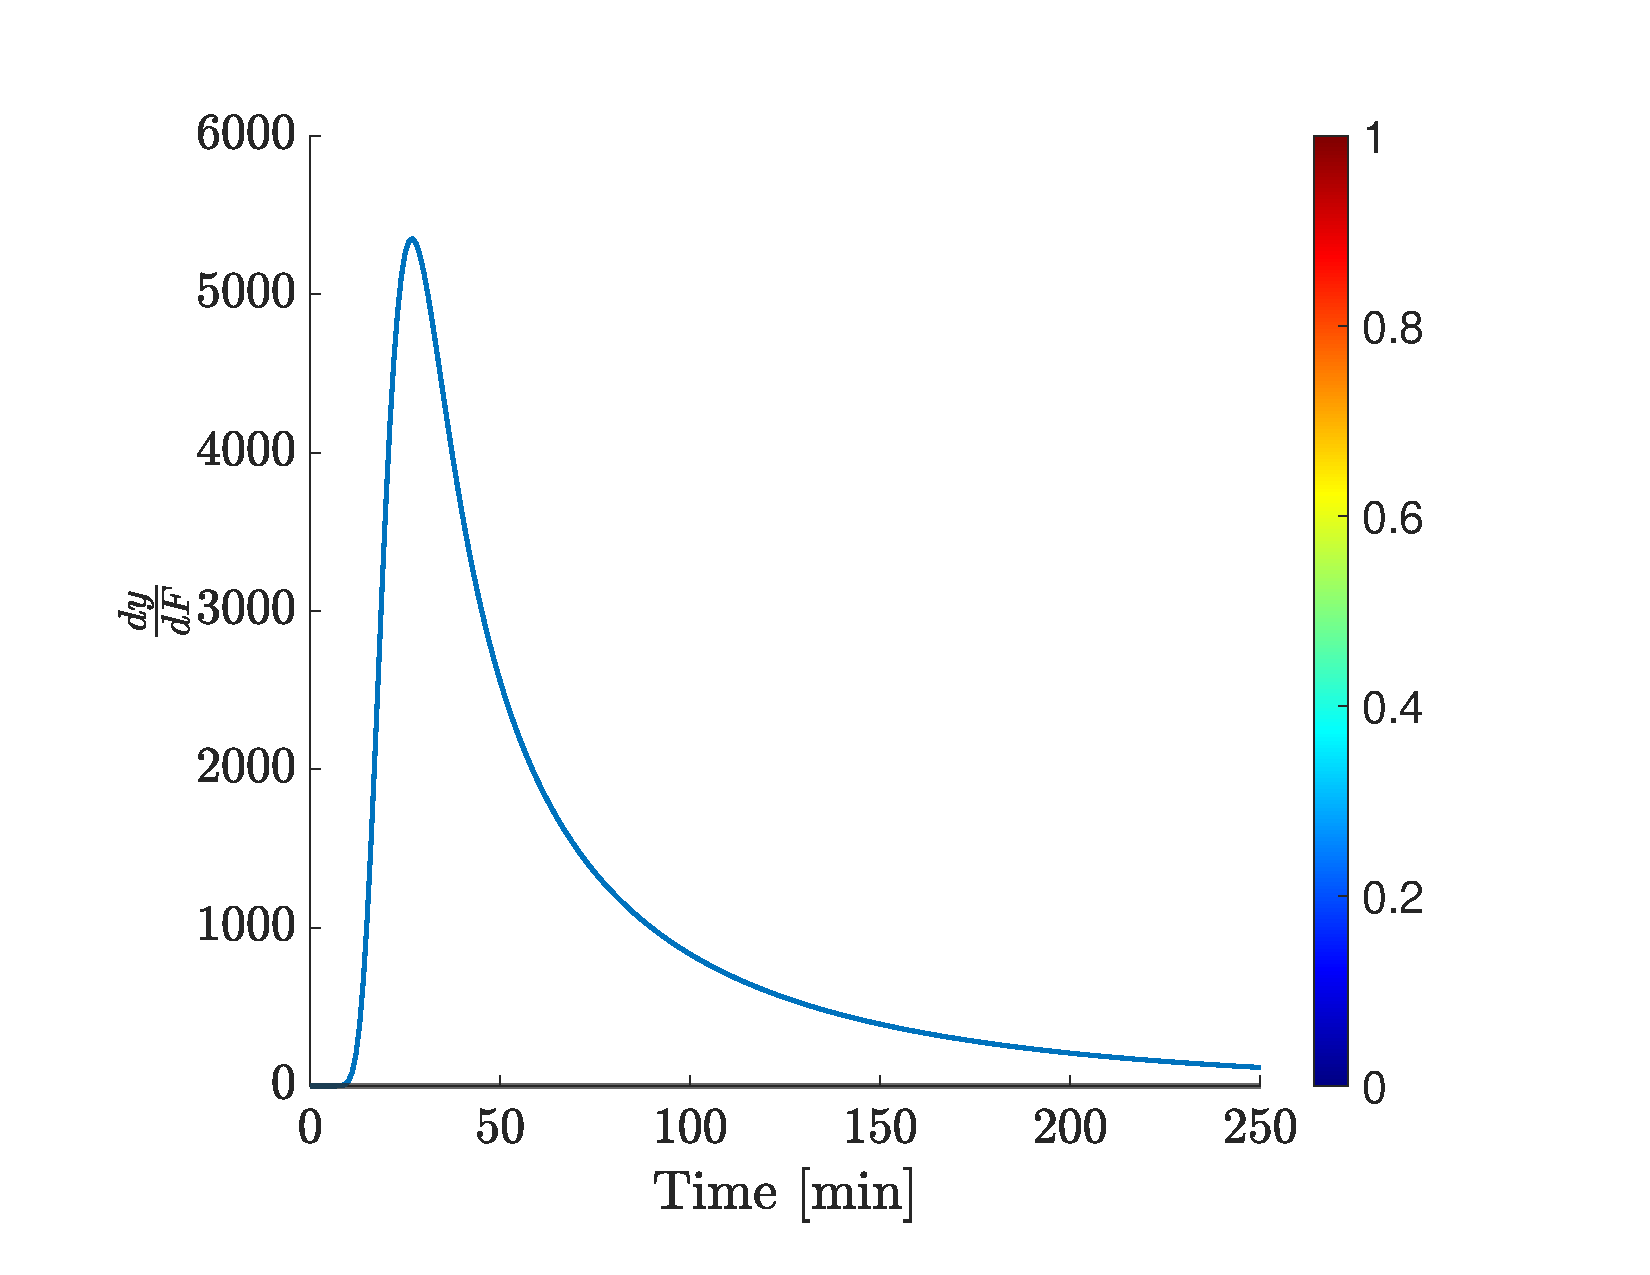
\includegraphics[trim = 2cm 0cm 0cm 0cm,clip,width=\columnwidth]{/Results_sensitivity/Y_F.pdf}
    	\caption{The effect of $F$ change on $y(t)$}
    	\label{fig:Sensitivty_F_y}
    \end{figure}
    
    \subsection{Pressure}
    
	
\end{document}